\documentclass{jsarticle} 
\usepackage[dvipdfmx]{graphicx} 
\usepackage[dvipdfmx]{hyperref}
\usepackage{amsmath}
\usepackage{color}
\usepackage{colortbl}
\usepackage{arydshln}
\usepackage{mathtools}

\newcommand*{\mbold}[1]{\mbox{\boldmath $#1$}}

%\renewcommand*{\labelenumi}{(\arabic{enumi})}

\newcommand*{\transp}[1]{\prescript{t\!}{}{#1}}

\newcommand*{\grad}{{\rm grad}}
\newcommand*{\divg}{{\rm div}}
\newcommand*{\rot}{{\rm rot}}
\newcommand*{\trace}[1]{{\rm tr}\!{#1}}


\title{Theorem1.32 : Stokes's Theorem}

\begin{document}
\maketitle

\begin{abstract}
  曲面$\mbold{S}(u, v)$状の, 閉曲線$C$を境界とする, 曲面領域$D$に対し, 
  $\mbold{S}$上で定義されている, ベクトル場$\mbold{A}$について, 以下が成立する. 
  \begin{eqnarray}
    \oint_C \mbold{A}\cdot d\mbold{r} = \int_D \rot \mbold{A} \cdot \mbold{n} dS
  \end{eqnarray}
\end{abstract}

\section{lemma1 : 線積分に対し, 積分途中に任意の往復を設けても結果が変わらない}
ある点$A$から$B$に向かう曲線$C$が, あるところで曲線$D$に接続されているとして, 
図のように, $A$から$B$に直接向かうのではなく, $B^\prime$で一旦$D$に乗換え, $B^{\prime\prime}$に一旦向かい, もう一度$B^\prime$に戻ってきて, 再び$B$へ向かう経路を考えたとする. 
\begin{figure}[htbp]
  \begin{center}
    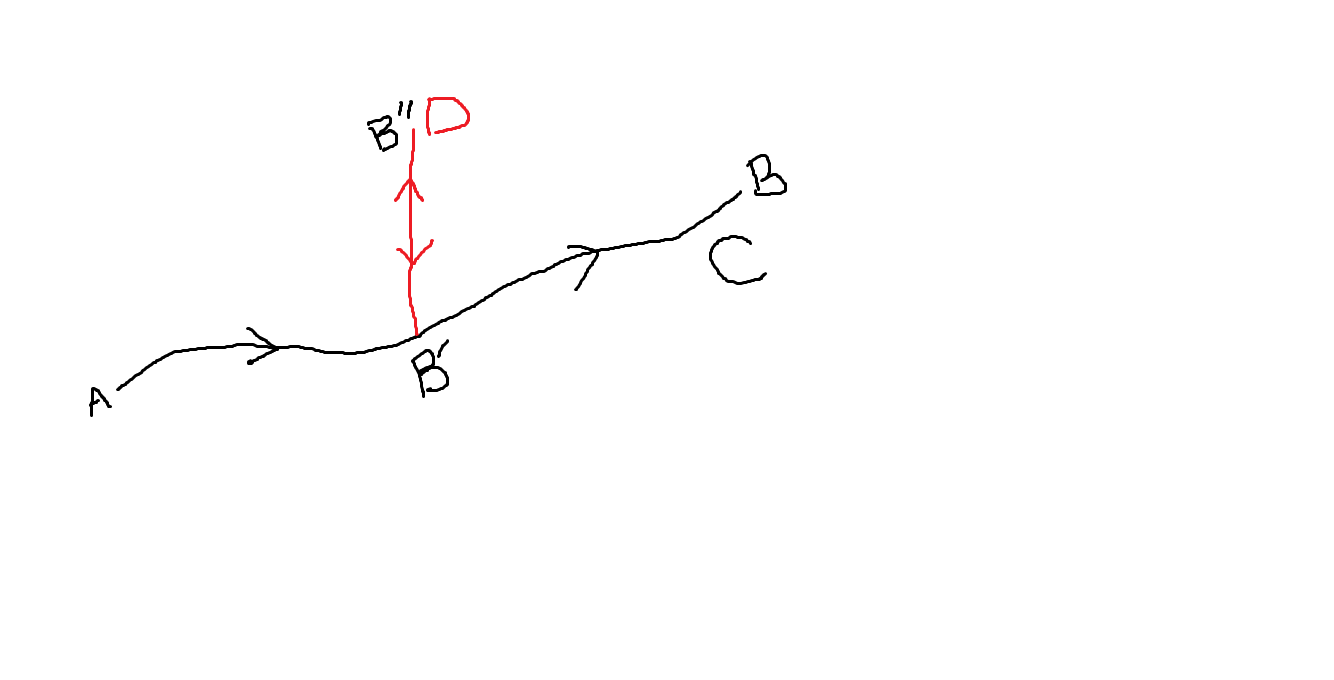
\includegraphics[width=10cm]{Figure/RouteAdd.png}
  \end{center}
\end{figure}

このとき, 全経路での線積分は, 
\begin{equation}
  \int_A^{B^\prime} \mbold{A}\cdot d\mbold{r} 
  + \int_{B^\prime}^{B^{\prime\prime}} \mbold{A}\cdot d\mbold{r} 
  + \int_{B^{\prime\prime}}^{B^\prime} \mbold{A}\cdot d\mbold{r} 
  + \int_{B^\prime}^B \mbold{A}\cdot d\mbold{r} 
\end{equation}
であるが, 線積分の性質により, 第二項, 第三項は打ち消しあうため, 結局, $C$のみでの積分と変わらない. 

\section{lemma2 : 閉曲線が囲む領域を分割すると, 元の閉曲線上での周回積分は, 各領域の境界線上での周回積分の和になる}
閉曲線$C$が囲む領域を, 図のように二分割する. 
\begin{figure}[htbp]
  \begin{center}
    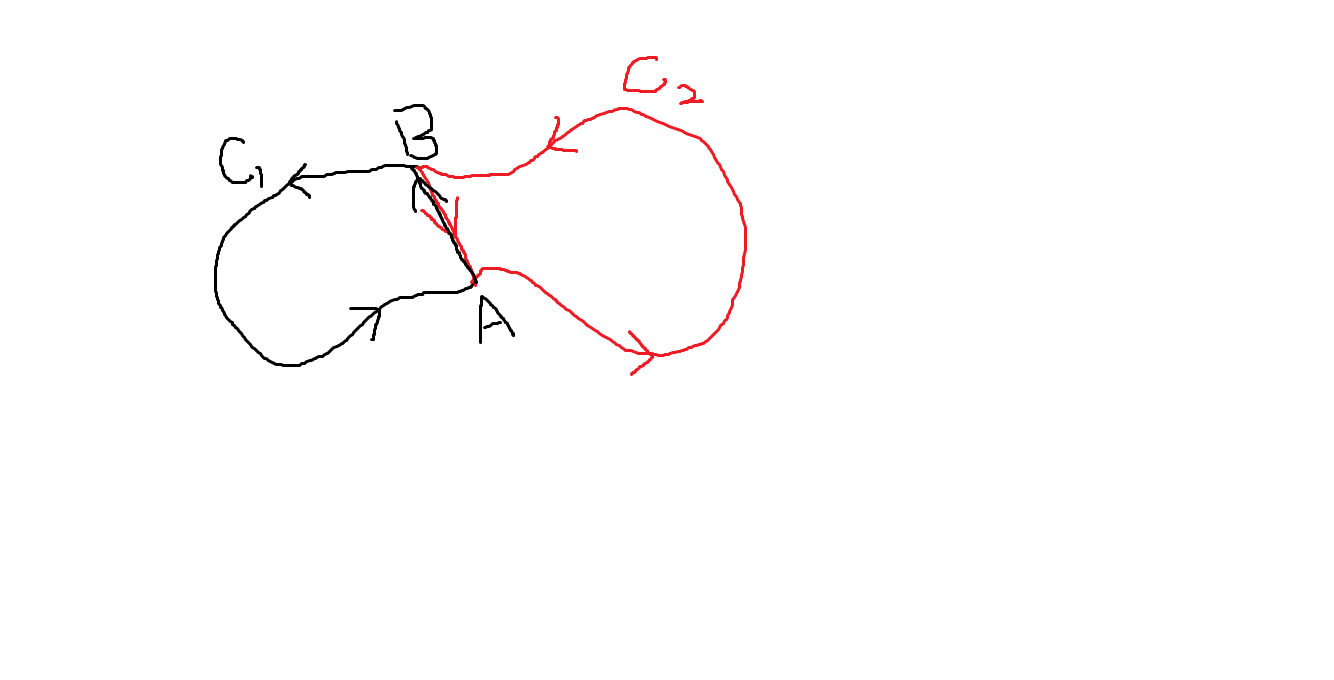
\includegraphics[width=10cm]{Figure/ClosedLoopDivide.png}
  \end{center}
\end{figure}

閉曲線$C$が, 点$B$から, $C_1$を経て, $A$を通って, $C_2$を経てまた$B$に向かう曲線であったと考えると, lemma1により, 本来の積分路である, $C_1$と$C_2$の間に, 
$A$から$B$に進んで, 再び, $B$から$A$に戻る, という往復を加えても結果は変わらない. 
従って, 
\begin{equation}
  \int_C \mbold{A}\cdot d\mbold{r}
  = \int_{C_1} \mbold{A}\cdot d\mbold{r} 
  + \int_{A}^{B} \mbold{A}\cdot d\mbold{r} 
  + \int_{B}^{A} \mbold{A}\cdot d\mbold{r} 
  + \int_{C_2} \mbold{A}\cdot d\mbold{r} 
\end{equation}

ここで, 第1, 2項に注目すると, $C_1$を経由し, $B$から$A$に向かったあと, $A$から再び$B$に向かうという積分路になっており, 
これはすなわち, 図の左側に分割された領域の周回積分である. 
同様に, 第3, 4項は, 右側の領域に関する周回積分である. 

このような操作と, 積分経路の分割を, 任意の回数続けていくことにより, $C$に囲まれた領域を任意の形状に分割することができ, 
全領域の周回積分の和, という形になる. 

\section{本証明}
対象となる領域$D$を, 境界が直交するように格子状に分割し, 一つの領域が, 局所的に平面とみなせるようにする. 
図のような, ある分割領域での周回積分を考える. 
\begin{figure}[htbp]
  \begin{center}
    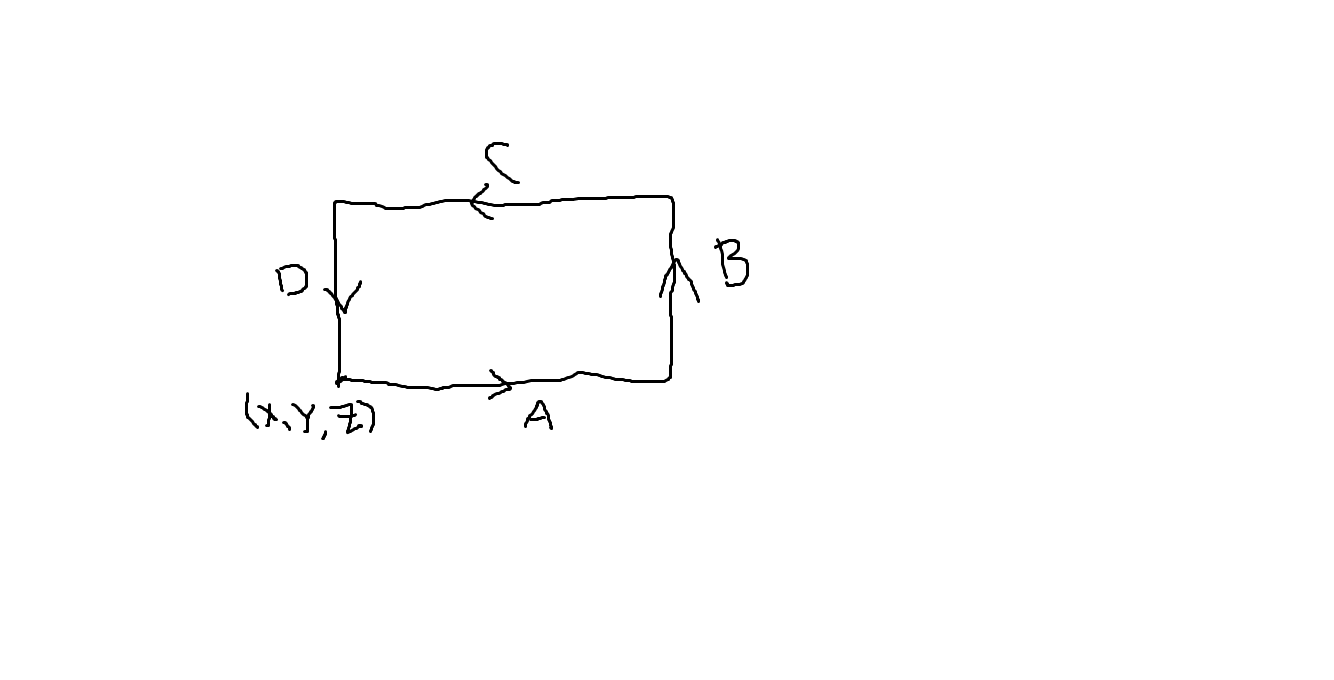
\includegraphics[width=10cm]{Figure/SmallArea.png}
  \end{center}
\end{figure}

このとき, 線積分の被積分関数は, 内積であるため, Theorem1.09により, 直交座標が相手であれば, 変換後の座標系でも計算結果は変わらない. 
従って, この格子のある点を原点とし, 直交する辺を, $x$軸, $y$軸となるような座標系で考える. 
経路に, 図のように名前を付けたとすると, この微少領域での線積分は, 
\begin{equation}
  \int_A \mbold{A}\cdot d\mbold{r} 
  + \int_B \mbold{A}\cdot d\mbold{r} 
  + \int_C \mbold{A}\cdot d\mbold{r} 
  + \int_D \mbold{A}\cdot d\mbold{r} 
\end{equation}
となる. 
第1項に注目すると, $d\mbold{r}$は, $x$軸しかないことを考慮すれば, 
\begin{equation}
  \int_A \mbold{A}\cdot d\mbold{r} = \int_x^{x + \Delta x}A_x(t, y, z)dt
\end{equation}
となる. 同様に, 
\begin{subequations}
  \begin{eqnarray}
    && \int_B \mbold{A}\cdot d\mbold{r} = \int_y^{y + \Delta y}A_y(x + \Delta x, t, z)dt \\
    && \int_C \mbold{A}\cdot d\mbold{r} = \int^x_{x + \Delta x}A_x(t, y + \Delta y, z)dt \\
    && \int_D \mbold{A}\cdot d\mbold{r} = \int^y_{y + \Delta y}A_y(x, y, z)dt
  \end{eqnarray}
\end{subequations}
となる. 
微少領域であるため, 例えば$A$上での$A_x$を, $(x, y, z)$周りで, 一次までTaylor展開すれば, 
\begin{equation}
  A_x(t, y, z) = A_x(x, y, z) + \frac{\partial A_x(x, y, z)}{\partial x}(t - x)
\end{equation}
となる. これをりようすれば積分は, 
\begin{equation}
  \int_x^{x + \Delta x}A_x(t, y, z)dt = A_x(x, y, z)\Delta x + \frac{\partial A_x(x, y, z)}{\partial x}\frac{\Delta x^2}{2}
\end{equation}
となり, 二次以上の項を無視すれば, 
\begin{equation}
  \int_x^{x + \Delta x}A_x(t, y, z)dt = A_x(x, y, z)\Delta x
\end{equation}
となる. 同様に, 
\begin{subequations}
  \begin{eqnarray}
    && \int_B \mbold{A}\cdot d\mbold{r} = A_y(x + \Delta x, y, z)\Delta y \\
    && \int_C \mbold{A}\cdot d\mbold{r} = -A_x(x + \Delta x, y + \Delta y, z)\Delta x \\
    && \int_D \mbold{A}\cdot d\mbold{r} = -A_y(x, y + \Delta y, z)\Delta y
  \end{eqnarray}
\end{subequations}
となる. 





\end{document}
